\chapter{Árvore de Objetivos}
Árvore de objetivos: é a representação gráfica do objetivo central do projeto (tronco), dos meios para alcançá-lo (raízes) e dos efeitos positivos que o alcance dos objetivos provoca na população-alvo (galhos e folhas). [7]

Tal ferramenta é importante para definição de objetivos claros a serem seguidos no projeto e auxiliam no desenvolvimento futuro do projeto.

A seguir pode-se ver a árvore de objetivos do presente projeto:

\begin{figure}
	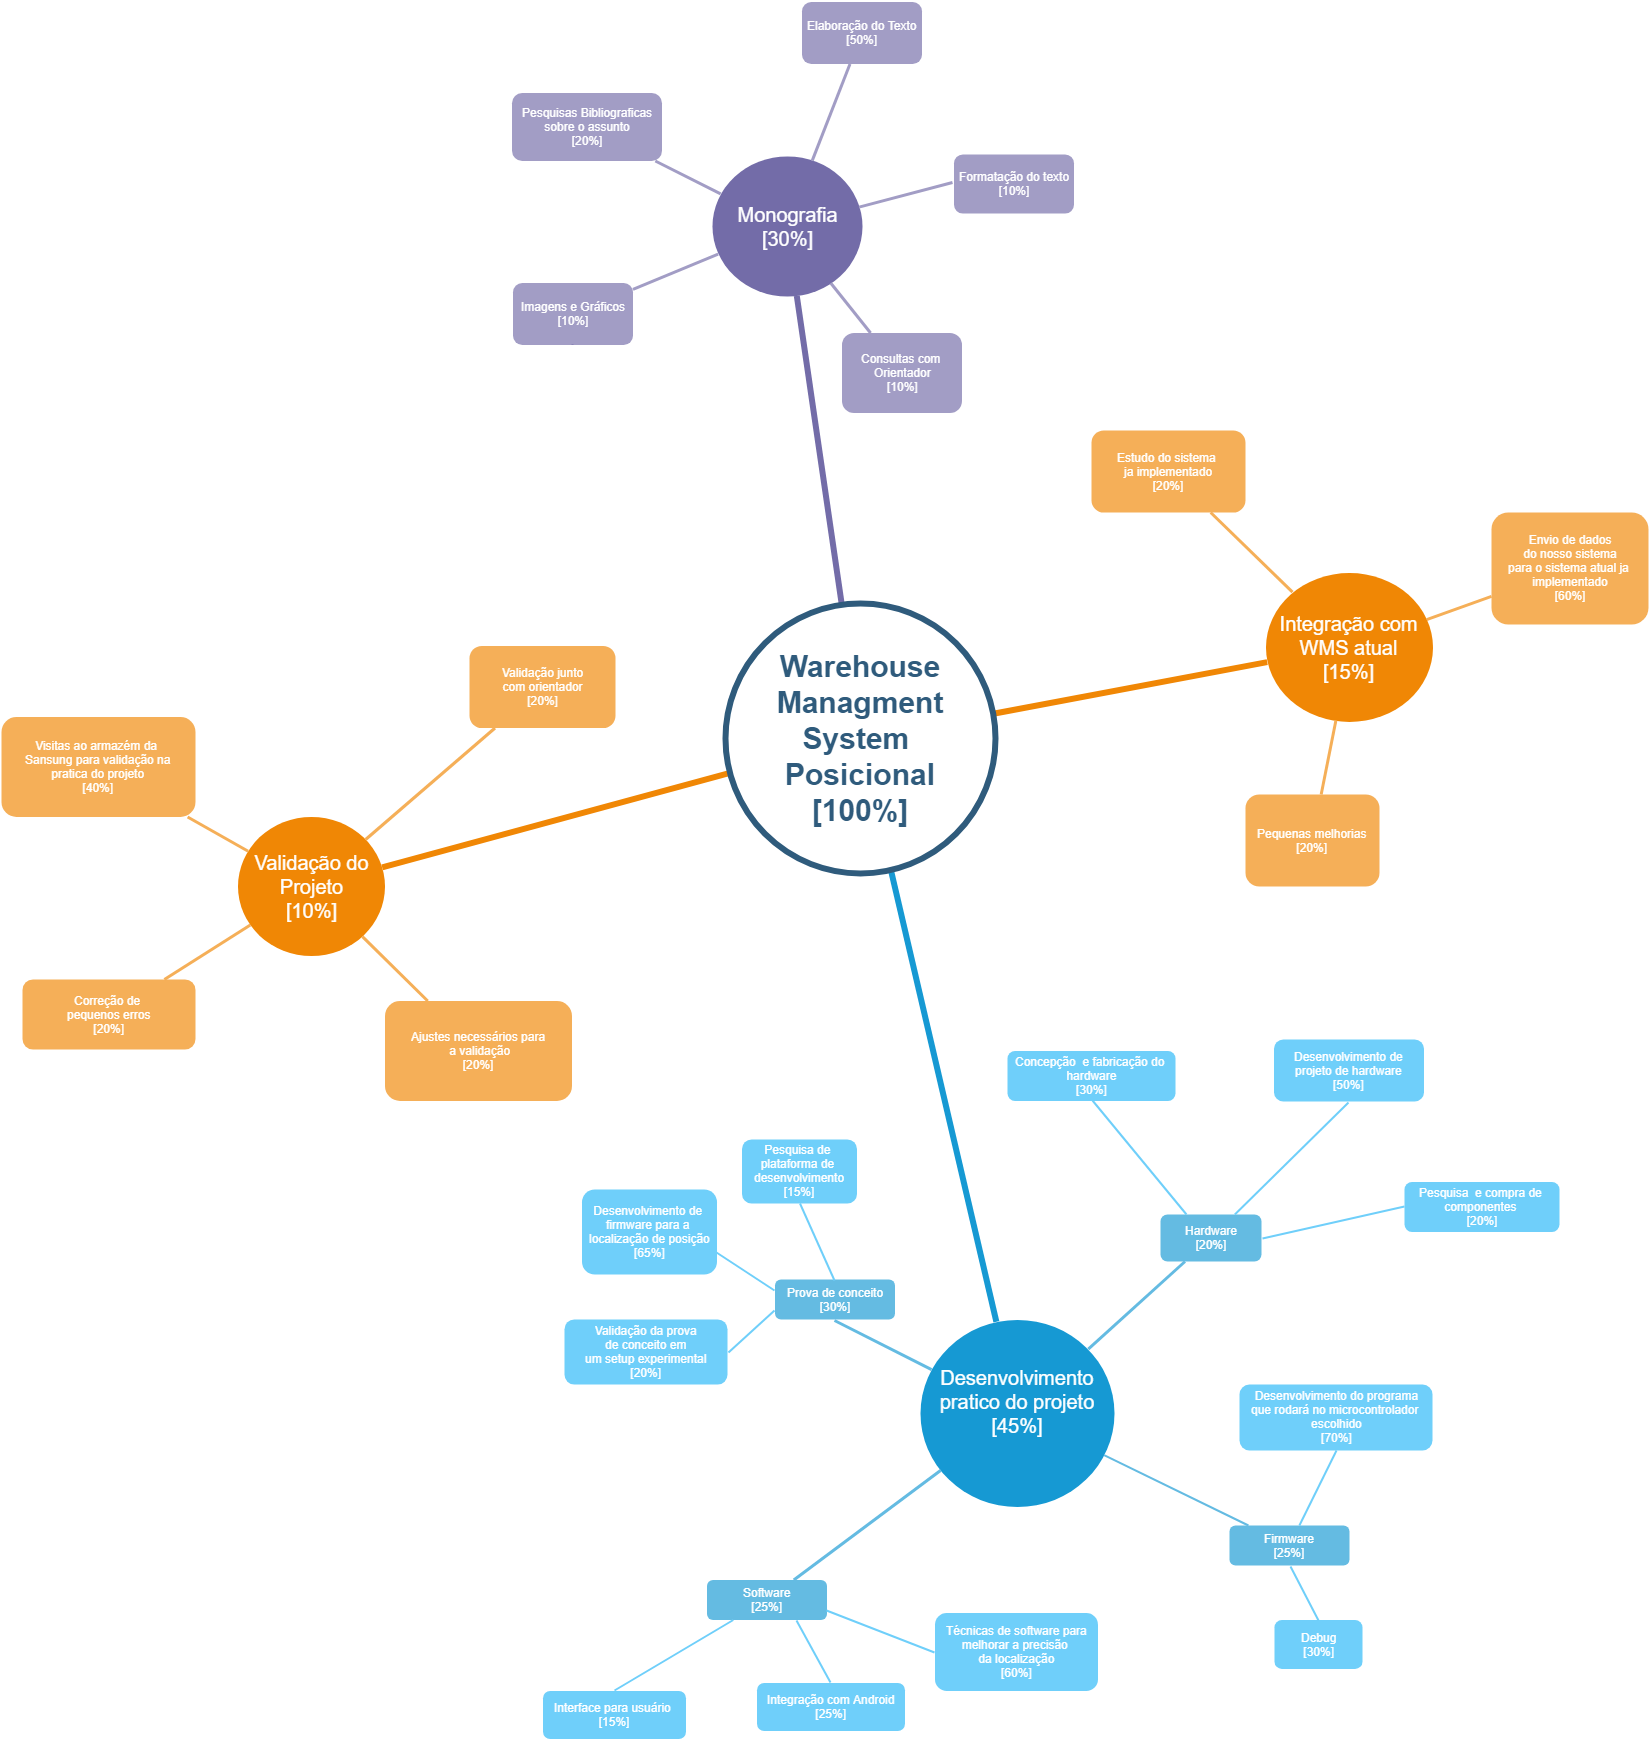
\includegraphics[width=\linewidth]{images/arvore_objetivos.png}
	\caption{Árvore de objetivos do projeto. Em colchetes os tempos de dedicação para cada parte}
	\label{fig:arvore_objetivos}
  \end{figure}